\subsubsection{x86}

\IFRU{Компилируем}{Let's compile} (MSVC 2010):

\lstinputlisting[caption=MSVC 2010]{\IFRU{14_bitfields/shifts_MSVC_ru.asm}{14_bitfields/shifts_MSVC_en.asm}}

\IFRU{Вот так работает SHL (\IT{SHift Left})}
{That's how SHL (\IT{SHift Left}) working}.

\IFRU{Скомпилируем то же и в}{Let's compile it in} GCC 4.4.1:

\lstinputlisting[caption=GCC 4.4.1]{14_bitfields/shifts_gcc.asm}

\IFRU{Инструкции сдвига также активно применяются при делении или умножении 
на числа-степени двойки ($1$, $2$, $4$, $8$, итд).}
{Shift instructions are often used in division and multiplications by power of two numbers 
($1$, $2$, $4$, $8$, etc).}

\IFRU{Например}{For example}:

\begin{lstlisting}
unsigned int f(unsigned int a)
{
	return a/4;
};
\end{lstlisting}

\IFRU{Имеем в итоге}{We got} (MSVC 2010):

\begin{lstlisting}[caption=MSVC 2010]
_a$ = 8							; size = 4
_f	PROC
	mov	eax, DWORD PTR _a$[esp-4]
	shr	eax, 2
	ret	0
_f	ENDP
\end{lstlisting}

\label{SHR}
\index{x86!\Instructions!SHR}
\IFRU{Инструкция \SHR (\IT{SHift Right}) в данном примере сдвигает число на 2 бита вправо. 
При этом, освободившиеся два бита слева (т.е., самые 
старшие разряды), выставляются в нули. А самые младшие 2 бита выкидываются. 
Фактически, эти два выкинутых бита ~--- остаток от деления.}
{\SHR (\IT{SHift Right}) instruction in this example is shifting a number by 2 bits right.
Two freed bits at left (e.g., two most significant bits) are set to zero.
Two least significant bits are dropped.
In fact, these two dropped bits ~--- division operation remainder.}

\index{x86!\Instructions!SHL}
\IFRU{Инструкция \SHR работает так же как и \SHL, только в другую сторону.}
{\SHR instruction works just like as \SHL but in other direction.}

\begin{figure}[ht!]
\centering
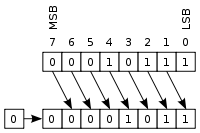
\includegraphics[scale=0.66]{14_bitfields/200px-Rotate_right_logically.png}
\caption{\IFRU{Как работает инструкция \SHR\protect\footnotemark}
{How \SHR instruction works\protect\footnotemark}}
\end{figure}

\footnotetext{\IFRU{иллюстрация взята из}{illustration taken from} wikipedia}

\label{division_by_shifting}
\IFRU{Для того, чтобы это проще понять, представьте себе десятичную систему счисления и число $23$. 
$23$ можно разделить на $10$ просто откинув последний разряд ($3$ ~--- это остаток от деления). 
После этой операции останется $2$ как частное
\footnote{результат деления}.}
{It can be easily understood if to imagine decimal numeral system and number $23$.
$23$ can be easily divided by $10$ just by dropping last digit ($3$ ~--- is division remainder). 
$2$ is leaving after operation as a quotient
\footnote{division result}.}

\IFRU{Так и с умножением. Умножить на $4$ это просто сдвинуть число на 2 бита влево, 
вставив 2 нулевых бита справа (как два самых младших бита). 
Это как умножить $3$ на $100$ ~--- нужно просто дописать два нуля справа.}
{The same story about multiplication.
Multiplication by $4$ is just shifting the number to the left by 2 bits,
while inserting 2 zero bits at right (as the last two bits).
It is just like to multiply $3$ by $100$ ~--- we need just to add two zeroes at the right.}


